\documentclass[a4paper,10pt]{article} 

\usepackage[utf8]{inputenc} 
%\usepackage[T1]{fontenc}

\usepackage{textcomp}           % Extra Symbole (Grad Celsius etc.)
\usepackage{amssymb,amsmath}    % Schöne Formeln (AMS = American Mathematical Society)
\usepackage{graphicx}           % Bilder und Seitenränder
\usepackage{subcaption}			% captions for subfigures
\usepackage{booktabs}           % Schönere Tabellen
\usepackage{colortbl}           % Farbige Tabellen

%\usepackage{tcolorbox}			% schöne bunte Boxen
\usepackage{mathtools}			% \mathclap für ordentliche \underbrace-			environments
\usepackage[left=2cm,right=2cm,top=2cm,bottom=2cm]{geometry}			% Pagelayout mit \newgeometry, \restoregeometry
\usepackage{float}
\usepackage{wrapfig}
\usepackage{enumitem}
\usepackage{float}
\usepackage{braket}
\usepackage{caption}
\usepackage[per-mode=reciprocal,output-decimal-marker={.},binary-units=true]{siunitx}
\usepackage[breaklinks=true,colorlinks=true,linkcolor=blue,urlcolor=blue,citecolor=blue]{hyperref} 
\usepackage{physics}
\usepackage{url}
\usepackage{subcaption}
\usepackage{calrsfs}
\DeclareMathAlphabet{\pazocal}{OMS}{zplm}{m}{n}

\graphicspath{{./img/}}

\newcommand{\dif}{\mathrm{d}}

\bibliographystyle{unsrtnat}

\renewcommand{\k}{\mathbf{k}}
\begin{document}
\begin{titlepage}
 \begin{center}
	\Large{Advanced laboratory class 3}
	\end{center}
	\begin{center}
	 \LARGE{\textbf{FP3 - SQUID}}
	\end{center}
	
	\begin{center}
	
	\large Marco \textsc{Canteri} \\
	marco.canteri@student.uibk.ac.at\\
	\large Maximilian \textsc{Münst} \\
	maximilian.muenst@student.uibk.ac.at
	\end{center}
	
	\begin{center}
	\vspace{1cm}
	Innsbruck, \today
	\vspace{1cm}
	\end{center}
	
	\begin{abstract}
    In the course of this experiment a look was taken at some basic properties of superconducturs and SQUIDs, like the current-voltage and the current-flux characteristics. Additionally, Shapiro-steps were observed from which the $e/h$-ratio can be calculated. Finally, the resistance of the SQUID was measured, dependent on the temperature. 
    \end{abstract}
    \vspace{1cm}
	
	\begin{center}
	
\includegraphics[scale=0.4]{img/uibk} 
	\end{center}

\end{titlepage}


\section{Introduction}
In most solid body physics courses one learns that the resistance of a substance is caused by electron scattering on obstacles like phonons, impurities in the lattice, or other electrons.\cite{grossmarx} This model predicts that the resistance decreases with decreasing temperature, but ultimately remains at a finite, non-zero value due to impurities in the lattice. 
However, in 1911 Heike Onnes discovered a drastic and unforeseen decrease in resistance of mercury at \SI{4.2}{\kelvin}, later terming the observed phenomenon superconduction. 
\begin{quote}
    Mercury has passed into a new state which, on account of its extraordinary electrical properties, may be called the superconductive state. \newline
    -- \textsc{Heike Kamerlingh Onnes}, according to \cite{grossmarx}
\end{quote} 
In 1933 Walther Meißner and Robert Ochsenfeld discovered that in addition to being perfect conductors, superconducting materials also are perfect diamagnets. Today, applications of superconduction range from Magnetic Resonance Imaging (MRI) in medicine to particle accelerators, where superconducting coils are used to generate powerful magnetic fields.\cite{grossmarx}

\section{Theoretical Background}

The theoretical introduction in this report is split into two parts, one being a general introduction to superconductivity, while the other one is about the Josephson Effect and its application in this experiment. The presented information us based on the ``Mr. SQUID''-manual \cite{skriptum} as well as the book ``\textit{Festkörperphysik}'' \cite{grossmarx}.

\subsection{Superconductivity}
Superconductivity is the property of a medium to conduct current without any resistance. It was first discovered in 1911, when Heike Onnes cooled down mercury below 4.2 K \cite{firstsuperconductor}, finding out that the resistance dropped to zero. Since this discovery, superconductivity has been discovered in many elements and media which resistance drops to zero below a particular critical temperature $T_c$. There are different ways to classify superconductors, the easiest one is to divide superconductors in low-$T_c$ and high-$T_c$ superconductors. Low temperature superconductors are material with a critical temperature below $30$ K, while high temperature superconductors have $T_c$ greater than 30 K.\\
Superconductors can lose their property of superconductivity not only with a change in temperature, but also with a change of magnetic field or current, this leads to a different classification of superconductors: type I and type II superconductors. The former has a critical external magnetic field $H_c$ and behaves as superconductor below this field. Type II superconductors have two different critical fields, and they behave differently in various regimes.\\
In this experiment we used a Yttrium barium copper oxide (YBCO) superconductor which is a high-$T_c$ superconductors, historically is also the first high-$T_c$ superconductors found with a critical temperature above 77 K, the boiling point of liquid nitrogen. Indeed the critical temperature of YBCO is around 90-94 K, depending of the compound and purity.\\
The theoretical description of superconductivity can be done in different ways, the first classical approach is the simplest description using London equations, a quantum mechanical formulation is the Ginzburg-Landau (GL) theory which describes the macroscopic properties of superconductors. However this theory is still phenomenological, the first microscopic model is the BCS theory which was able to describe superconductivity from a microscopic point of view and has the GL theory as a limit. The key idea of BCS theory is that at low temperatures electrons pair up and form Copper pairs, creating a bosonic condensate. This condensate must be described as a single entity with a wavefunction $\psi(\mathbf{r},\theta) = |\psi(\mathbf{r})| e^{i\theta}$, which is not normalized, but $|\psi(\mathbf{r},\theta)|^2 = n_e$, where $n_e$ is the number of electrons in the superconductive state. These theory predicts the behaviour of low temperature superconductors, but fails to describe high temperature superconductors, whose description is still an open problem.

\subsection{Josephson Effect and SQUID} % AC, DC Josephson effect & Shapiro steps, SQUID 

\subsubsection*{DC Josephson Effect}
The Josephson effect is caused by the long range quantum interaction in superconductors. The junction itself can be seen as a gap or barrier between two superconductors as is sketched in Fig. \ref{figure_josephson_junction}. In the Mr. SQUID \cite{skriptum} device, the junctions are grain boundary weak-link junctions. 

\begin{figure}[htp!]
    \centering
    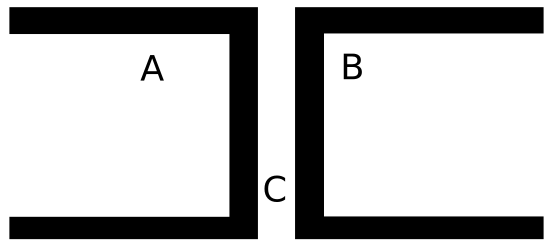
\includegraphics[width = 0.6 \textwidth]{josephson.png}
    \caption{Sketch of a Josephson junction. The wavefunctions with respective phases $\varphi_A$ and $\varphi_B$ interfere over the barrier C.}
    \label{figure_josephson_junction}
\end{figure}

The supercurrent flowing through the junction is dependent on the density of electron-electron pairs or Cooper pairs $n_{S,A}$ and $n_{S,B}$, the phases of the two macroscopic wave functions $\Psi_A$ and $\Psi_B$ and the properties of the junction. Assuming that the coupling is small, it follows that $\abs{\Psi_A}^2 = n_{S,A}$ and $\abs{\Psi_B}^2 = n_{S,A}$ remain approximately constant and should have the same value $n_{S}$. 
According to \cite{grossmarx}, the most general expression for the supercurrent density is then 
\begin{equation}
    J_S = q_S n_S(\vec{r},t) \big[ \frac{\hbar}{m_S} \nabla \Theta(\vec{r},t) - \frac{q_S}{m_S} \vec{A}(\vec{r},t) \big] = \frac{q_S n_S \hbar}{m_S} \vec{\gamma}(\vec{r},t)
\end{equation}
with $\vec{\gamma}(\vec{r},t) = \nabla \Theta - \frac{2 \pi}{\Phi_0} \vec{A}(\vec{r},t)$. It is fair to assume that the phase gradient in the barrier is big compared to the gradient in the superconductor. Assuming further that the phase gradient $\vec{\gamma}$ is constant over the small junction, one can introduce a gauge invariant phase difference $\phi(\vec{r}, t)$ as 
\begin{equation}
    \begin{split}
        \label{eq_phase}
        \varphi(\vec{r}, t) &= \int^B_A \vec{\gamma}(\vec{r},t) = \int^B_A \big[ \nabla \Theta - \frac{2 \pi}{\Phi_0} \vec{A}(\vec{r},t) \big] \dif \vec{l} \\
        &= \Theta_B(\vec{r}, t) - \Theta_A(\vec{r}, t) - \frac{2 \pi}{\Phi_0} \int^B_A \vec{A}(\vec{r},t) \dif \vec{l}
    \end{split}
\end{equation}

According to \cite{skriptum}, the supercurrent $I_S$ solely depends on the phase difference $\varphi$. Furthermore, the wave functions $\Psi_A$ and $\Psi_B$ have to be invariant under a phase change of a multiple of $2 \pi$. 
\begin{equation}
    I_S(\varphi) = I_S(\varphi + n 2 \pi)
\end{equation}
Also, if there is no supercurrent in the superconductor, the phase difference has to be $0$. Hence, one can write 
\begin{equation}
    I_S(\varphi = 0) = 0 = I_S( n 2 \pi).
\end{equation}
Combining these results leads to sinusodial dependence of the supercurrent $I_S$ on the phase difference $\phi$.
\begin{equation}
    I_S(\varphi) = I_C \sin(\varphi) + \underbrace{\sum^{\infty}_{m = 2} I_m \sin(m \varphi)}_{\approx 0}
    \label{first_josephson}
\end{equation}
Eq. \ref{first_josephson} is often referred to as the first Josephson equation. The higher order terms are often ignored as they are usually very small. 

The second Josephson equation can be calculated from the time derivative of Eq. \ref{eq_phase}, which is 
\begin{equation}
    \pdv{\varphi}{t} = \pdv{\Theta_B}{t} - \pdv{\Theta_A}{t} - \frac{2 \pi}{\Phi_0} \pdv{}{t} \int^B_A \vec{A}(\vec{r},t) \dif \vec{l}.
\end{equation}
Using the energy-phase relation form \cite{grossmarx}, which is given as 
\begin{equation}
    -\hbar \pdv{\Theta}{t} = \frac{1}{2 n_S} \Lambda \vec{J_S}^2 + q_S \phi + \mu,
\end{equation}
where $\Lambda = \frac{m_S}{n_S q_S^2}$ is the London coefficient, $q_S = -2 e$ is the charge of a Cooper pair, $\phi$ is a gauge scalar field and $\mu$ is the chemical potential. This yields the following expression:
\begin{equation}
    \pdv{\varphi}{t} = - \frac{1}{\hbar} \big( \frac{\Lambda}{2 n_S} \underbrace{[\vec{J}_S^2(B) - \vec{J}_S^2(A)]}_{ = 0} + q_S [\phi(B) - \phi(A)] + [\mu(B) - \mu(A)] \big) -  \frac{2 \pi}{\Phi_0} \pdv{}{t} \int^B_A \vec{A}(\vec{r},t) \dif \vec{l}
\end{equation}
Continuity requires that the currents at both sides of the junction are equal in size. This then leads to the second Josephson equation:
\begin{equation}
\pdv{\varphi}{t} = \frac{2 \pi}{\Phi_0} \int^B_A \big[ - \nabla \tilde{\phi} - \pdv{\vec{A}}{t} \big] \dif \vec{l} = \frac{2 \pi}{\Phi_0} \int^B_A \vec{E}(\vec{r},t) \dif \vec{l} = \frac{2 \pi}{\Phi_0} U,
\end{equation}
where $U$ is the voltage over the junction. It follows that the phase increases with time, resulting in 
\begin{equation}
    \varphi(t) = \varphi_0 + \frac{2 \pi}{\Phi_0} U t.
    \label{eq_josephson_2}
\end{equation}

\subsubsection*{AC Josephson Effect} % AC & Shapiro Steps
If one now adds an alternating current to the DC voltage $U = U_0 + U_1 \sin(\omega_1 t)$ in Eq. \ref{eq_josephson_2}, one gets 
\begin{equation}
    \varphi(t) = \varphi(0) + \frac{2 e U_0}{\hbar} t + \frac{2 e U_1}{\hbar \omega_1} \sin(\omega_1 t).
\end{equation}
This expression can now be inserted into the first Josephson equation, which yields 
\begin{equation}
    I_S(\varphi) = I_C \sin \big( \varphi(0) + \frac{2 e U_0}{\hbar} t + \frac{2 e U_1}{\hbar \omega_1} \sin(\omega_1 t) \big). 
\end{equation}
Using the first order Bessel function $\pazocal{J}$, one can write
\begin{equation}
    J_S(t) = J_C \sum^{\infty}_{n = 0} \pazocal{J}_n \big[ \frac{2 e U_1}{\hbar \omega_1} \big] \underbrace{\sin \big( \varphi(0) + \frac{2 e U_0}{\hbar} t \pm n \omega_1 t \big)}_{= const \Leftrightarrow U_0 = n \frac{\hbar \omega_1}{2e}}.
\end{equation}
Since one usually measures the DC components in the experiment, one has to find the DC voltage at which the sine becomes time-independent. This is true for $U_0 = n \frac{\hbar \omega_1}{2e}$. If one measures the $I$-$V$ characteristic of a Josephson junction, one will see steps in the curve. The height of the steps is determined by the amplitude of the alternating current $U_1$ and the corresponding Bessel function $\pazocal{J}_n$. They are often called Shapiro steps.

\subsubsection*{Superconducting QUantum Interference Device - SQUID}
A simple circuit diagram of a SQUID is displayed in Fig. \ref{fig_squid}. It shows that the Josephson junctions are set up in a parallel way and are connected with superconducting material. Assuming that the critical current $I_C$ is equal for both junctions, one can use the phase-current relation from \cite{grossmarx}, which says that the currents in then junctions can be expressed as $I_{S,1}=I_C \sin(\varphi_1)$ and $I_{S,2} = I_C \sin(\varphi_2)$.
\begin{figure}[htp!]
    \centering
    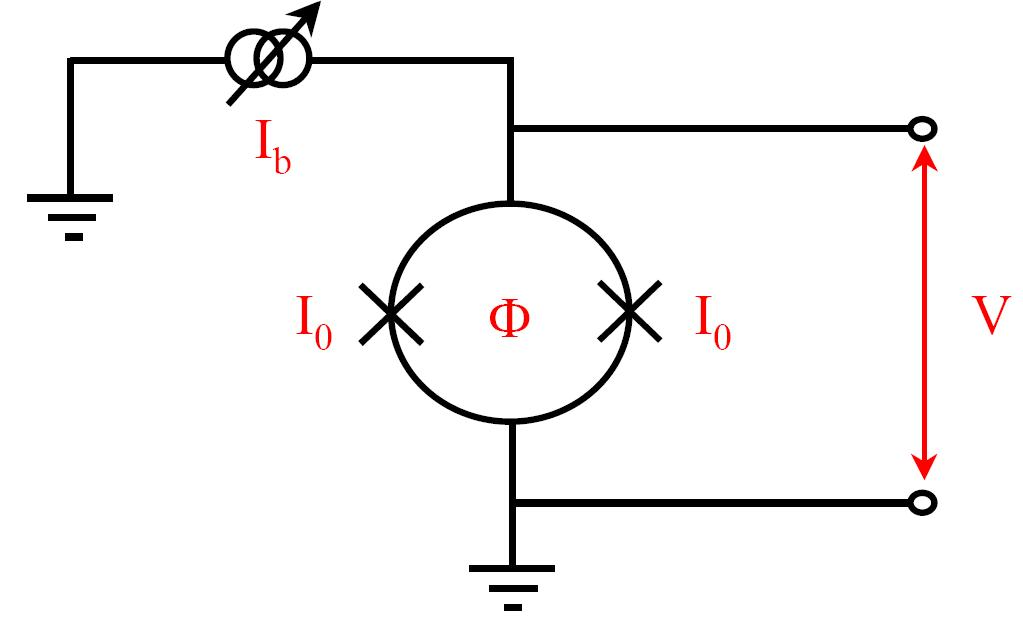
\includegraphics[width = 0.6 \textwidth]{SQUID_IV.jpg}
    \caption{Schematic of a DC SQUID, taken from \cite{squid_circuit}. An input bias current $I_b$ produces a voltage over the two parallel arranged Josephson junctions, through which a current $I_0$ is passing. If one now adds a magnetic flux $\Phi$ through the SQUID, an additional current $I_S$ is induced, which is running circular in the SQUID, adding to the bias current in the Josephson junctions. This induced current reduces the critical current of the SQUID.}
    \label{fig_squid}
\end{figure}
Using Kirchhoff's law and the addition theorems, one can write the total current as 
\begin{equation}
    \label{eq_continuity}
    I_S = I_{S,1} + I_{S,2} = 2 I_C \cos(\frac{\varphi_2 - \varphi_1}{2}) \sin(\frac{\varphi_1 + \varphi_2}{2})
\end{equation}
According to \cite{grossmarx}, one can further argue that in the total phase change across the ring, the phase change in the superconductor is negligible compared to the change in the Josephson junctions. Therefore, one can reach the following equation using Eq. \ref{eq_phase}. 
\begin{equation}
    \varphi_1 - \varphi_2 = - \frac{2 \pi}{\Phi_0} \underbrace{ \oint \vec{A} \dif \vec{l} }_{= \Phi}
\end{equation}
Here $\Phi$ is the flux through the SQUID. Inserting this into Eq. \ref{eq_continuity} leads to 
\begin{equation}
    I_S^\mathrm{max} = 2 I_C \cos(\frac{\pi \Phi}{\Phi_0}) \sin(\varphi_1 + \frac{\pi \Phi}{\Phi_0}) \stackrel{\Phi = \Phi_\mathrm{ext}}{=} 2 I_C \abs{\cos \big( \frac{\pi \Phi_\mathrm{ext}}{\Phi_0} \big)}.
\end{equation}
This equation finally shows the critical maximum the supercurrent can reach when a magnetic field is applied on the SQUID. $I_C$ in this equation means the critical current per junction, which is half the critical current of the SQUID. 

\section{Experimental Setup}

\subsection{The $V$-$I$ characteristics}
\label{setup_vi}
The first part of the experiment was the measurement of the $V$-$I$ characteristics. In order to conduct this measurement the SQUID probe was first connected to the control box and then inserted into a bath of liquid nitrogen in order to cool down below the critical temperature $T_C$. Measurements above $T_C$ were conducted only in the last part of the experiment. 
The lever on the control box is switched to $V$-$I$ mode, the FLUX and BIAS OFFSET are both turned into 12-o'clock position, the SWEEP OUTPUT is put at the zero position. Then the BIAS is tuned to what was estimated to be the center position in the $V$-$I$ characteristic curve on the oscilloscope. Then the SWEEP OUTPUT was gradually increased. In $V$-$I$ mode the SWEEP varies the BIAS OFFSET so one can actually see a characteristic curve on the oscilloscope. However, one has to consider that the output of the control box, which is visible on the oscilloscope is amplified by a factor of $\num{e4}$.\cite{skriptum} 
To vary the critical current one can in a final step change the FLUX OFFSET. This causes the $I_C$ to oscillate between a minimum and a maximum. For several FLUX settings the $V$-$I$ characteristics were recorded and are further discussed in the analysis.

\subsection{The $V$-$\Phi$ characteristics}
In the following part the $V$-$\Phi$ characteristics had to be recorded. Continuing from the previous setup, the FLUX setting was adjusted to where the critical current reaches a maximum. In a next step the SWEEP was put to zero, so that only a point was visible on the oscilloscope. Using BIAS this point was positioned right at the ´´knee'' of the $V$-$I$ characteristic curve. 
Next, the mode of the control box was changed to $v$-$\Phi$ mode. In this setting the SWEEP OUTPUT does not affect the BIAS but the FLUX OFFSET. One can now increase the SWEEP, which results in a sinusodial curve on the oscilloscope. These curves are saved and again displayed and discussed in the analysis.  

\subsection{Shapiro steps and $e/h$}
In order to observe Shapiro steps, we inserted an antenna inside the dewar such that we coupled electromagnetic radiation with the squid. The antenna was connected to a function generator with we used to generate a sine wave whit variable amplitude and frequency. With this setup we acquired again the characteristic V-I curve of the SQUID for five different frequencies ranging from 10 to 20 GHz. After setting the desired frequency we changed the power of the wave such that the Shapiro steps were maximized.
\subsection{Critical temperature measurement}
To measure the critical current of the SQUID we measured the resistance at various temperatures. To measure the temperature we build the circuit in figure \ref{circuit}. The REF02 provides us with a stable voltage of approximately 5V, we chose resistor $R_1 \simeq 40$ k$\Omega$ and $R_2 \simeq 10$ k$\Omega$ such that the voltage at the non inverting input of the opamp is around 1V. For the last resistor  we chose $R_3 \simeq 80$ k$\Omega$, thus the fixed current was approximately 12 mA. The diode was attached to the squid, hence we were able to measure a difference in temperature by measuring the voltage across the diode. To calibrate this circuit we took two points, one at the boiling point of the nitrogen (77 K) and the other one at room temperature, such that we had a direct conversion from voltage to temperature.\\
To measure the resistance of the SQUID we acquired the characteristic V-I curve whose slope gives the resistance. We proceeded to slowly lower the squid into the liquid nitrogen, such that the gradient of temperature between the liquid nitrogen and the environment would give us different points with different temperatures. During the lowering we stopped several times to take the measurements, every time we waited several minutes until voltage on the multimeter was stable and then we acquired the resistance and wrote down the voltage on the multimeter.
We took several point with different spacing, more densly near the critical temperature at 90 K and more rarely at higher temperature until the squid was completely inside the liquid nitrogen and therefore at 77 K.
\begin{figure}[H]
\centering
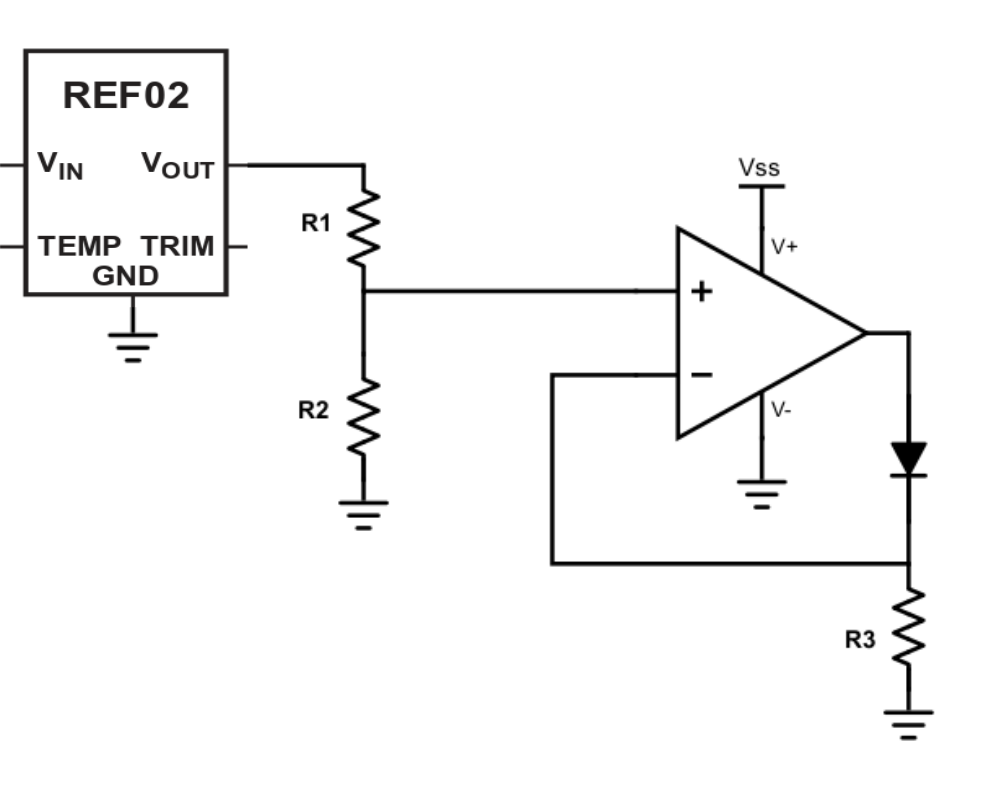
\includegraphics[width = .5\textwidth]{circuit}
\caption{Circuit for current source used to measure the temperature}\label{circuit}
\end{figure}

\section{Analysis}
\subsection{The $V$-$I$ characteristics}
As was already described in Sec. \ref{setup_vi}, the characteristic $V$-$I$ curve was measured in the first part of the experiment. Fig. \ref{fig_iv_characteristics} displays two $V$-$I$ characteristics. The left curve shows the maximum value of $I_C$ that was measured during the experiment, which means that the flux was at that point an integer multiple of the fluxon $\Phi_0$. On the right one can see the minimized $I_C$, which corresponds to an integer plus $1/2$ multiple of $\Phi_0$. 
\begin{figure}[htp!]
    \centering
    \begin{subfigure}[t]{0.45 \textwidth}
        \centering
        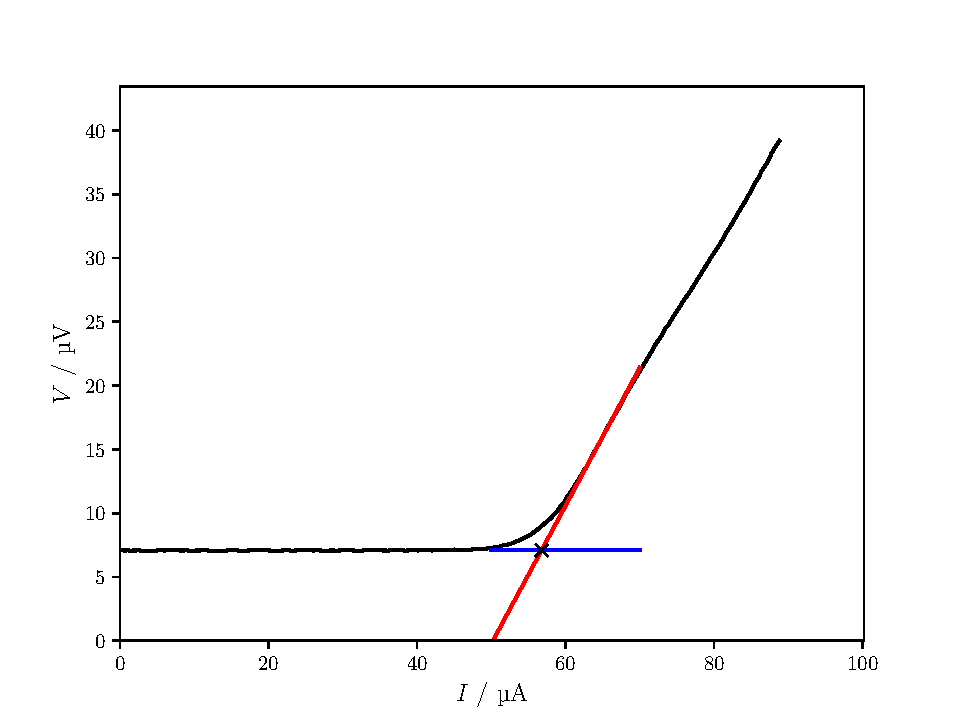
\includegraphics[height=6cm]{iv_max.pdf}
        \caption{ }
    \end{subfigure}
    ~ 
    \begin{subfigure}[t]{0.45 \textwidth}
        \centering
        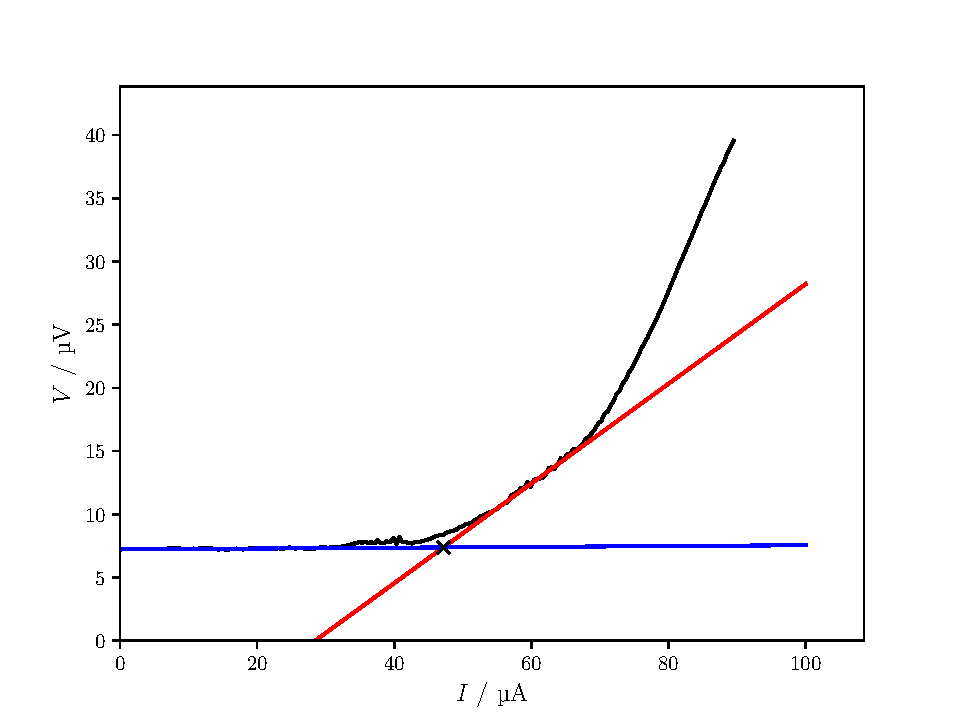
\includegraphics[height=6cm]{iv_min.pdf}
        \caption{ }
    \end{subfigure}
    \caption{Measured $V$-$I$ characteristics for an integer and an integer plus $1/2$ magnetic flux. The parameters of the linear functions are listed in Tab. \ref{tab_iv_characteristics}. The resulting critical currents are $I_C^{max} = \SI{56.8(8)}{\micro \ampere}$ and $I_C^{min} = \SI{47.2(17)}{\micro \ampere}$. }
    \label{fig_iv_characteristics}
\end{figure}
\begin{table}[htp!]
    \caption{List of the fit parameters from Fig. \ref{fig_iv_characteristics}. The fitted function was $V = a I + b$}
    \centering
    \begin{tabular}{l | l | l | l}
        max/min $I_C$ & color & $a$ & $b$ \\ \hline
        $I_C^{max}$ & red & \SI{1.082(11)}{\micro \volt \per \micro \ampere} & \SI{-54.3(7)}{\micro \volt} \\ 
        $I_C^{max}$ & blue & \SI{0.0006(109)}{\micro \volt \per \micro \ampere} & \SI{7.1(7)}{\micro \volt} \\
        $I_C^{min}$ & red & \SI{0.394(9)}{\micro \volt \per \micro \ampere} & \SI{-11.2(5)}{\micro \volt} \\
        $I_C^{min}$ & blue & \SI{0.00328(19)}{\micro \volt \per \micro \ampere} & \SI{7.230(3)}{\micro \volt}
    \end{tabular}
    \label{tab_iv_characteristics}
\end{table}
From the fit parameters the critical currents are deduced as $I_C^{max} = \SI{56.8(8)}{\micro \ampere}$ and $I_C^{min} = \SI{47.2(17)}{\micro \ampere}$. From the difference between these two values, one can derive the screening current as $I_S = I_C^{max} - I_C^{min} = \SI{9.6(19)}{\micro \ampere}$. 

To determine the normal resistance $R_n$ one takes a data set with a wide range of $I$ values as is depicted in Fig. \ref{fig_resistance}. The slope of the linear fit across the data corresponds to the normal resistance $R_n = \SI{0.6747(2)}{\ohm}$, which is reasonably close to the \SI{0.64}{\ohm} that are given in the data sheet.\cite{datasheet} 

\begin{figure}[htp!]
    \centering
    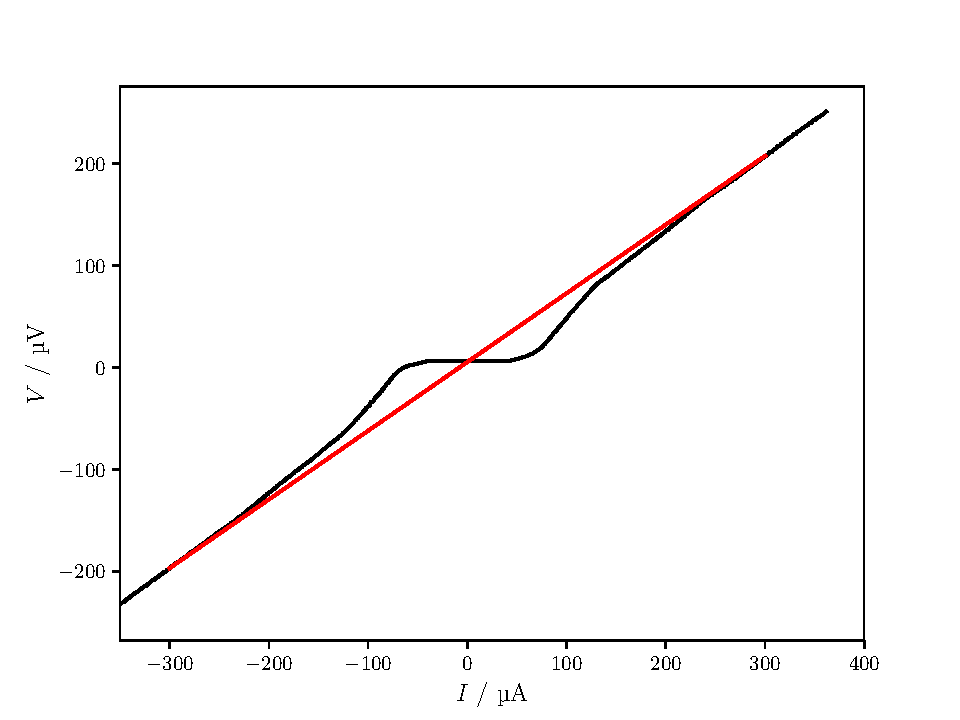
\includegraphics[width = 0.6 \textwidth]{resistance.pdf}
    \caption{Wide range $V$-$I$ characteristic curve. From the linear fit with parameters $a = \SI{0.6747(2)}{\ohm}$ and $b = \SI{5.36(7)}{\micro \ampere}$ the resistance $R_n = a$ can be deduced. }
    \label{fig_resistance}
\end{figure}
% still missing the \beta_L shit ...
\subsection{The $V$-$\Phi$ characteristics}
\subsection{Shapiro steps and $e/h$}
\begin{figure}[H]
\centering
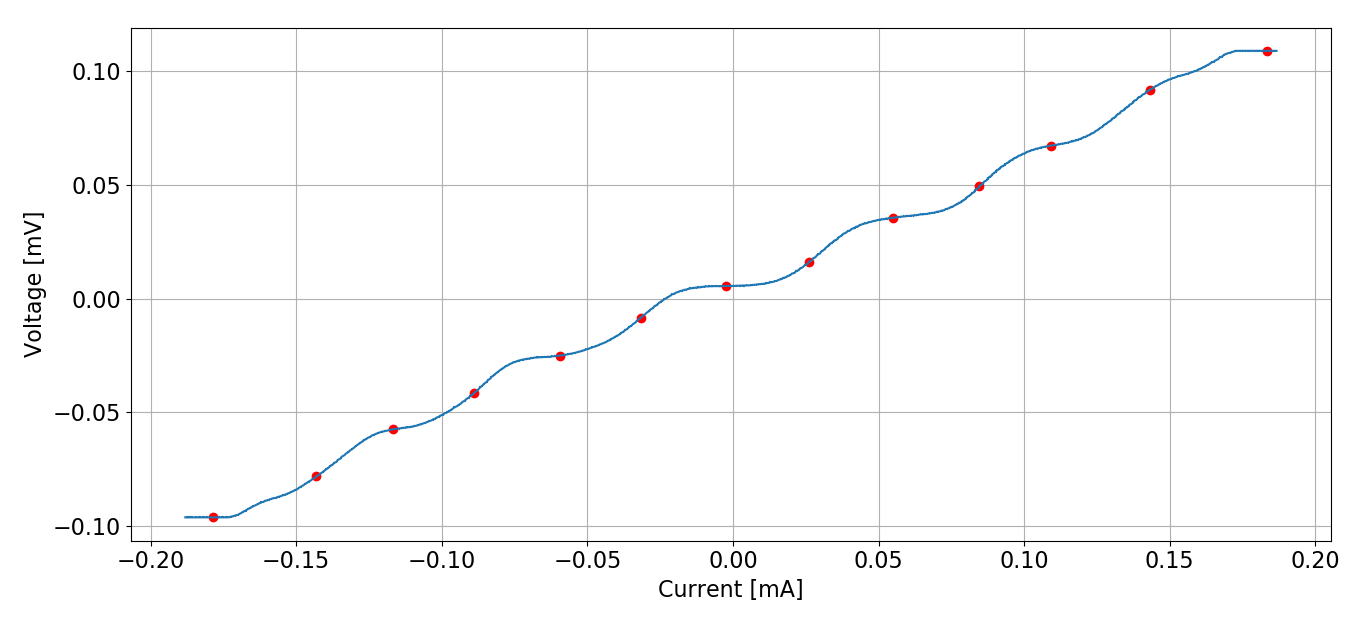
\includegraphics[width = \textwidth]{shapirosteps}
\caption{Shapiro steps for frequency of 15 GHz, red points are the calculated inflection points. Errors are too small to be seen}\label{shapiro}
\end{figure}
Due to the SWEEP OUTPUT the line sweep several time from left to right and vice versa, so we exploited this excess of data to smooth the line and calculate an error for every point. First we sorted the data in the characteristic curve, then we averaged over 10 neighbor points. The final curve is the set of all the averages and the standard deviation used as an error, an example of acquired data is shown in figure \ref{shapiro}. The next step in the analysis is to find the steps in the curve, a task not trivial. We identify a step as an inflection point in our data. The approach we used to find the inflection point was to interpolate the data with a spline for which is easy to find the inflection point, then after finding the inflection points on the spline, we took the closer points of the data to the calculate inflection points. The result of this algorithm can be seen in figure \ref{shapiro}.\\
To calculate the step height we took as many steps as it was possible for every frequency, calculated the difference in height between these steps and then divided by the number of steps taken, such that the error is minimized. The step height for every frequency can be seen in figure \ref{eh}, the error is calculated with propagation on the difference between two point and then is divided by the number of steps taken. From the theory we know that the height of one step should be
\[V_0 = \frac{h\nu}{2e},\]
hence, we did a linear regression on the data in figure \ref{eh} to find the slope $h/2e$. The point at 20 GHz was excluded since it is several standard deviations aways from what we expected, likely due to an unknown error or maybe a problem in the inflection point detection algorithm. The regression gave the value $0.00208\pm 0.8\cdot 10^5$ mV for the slope with a reduced chi squared of $\chi_\nu \simeq 75$, thus we find $e/h = 24010 \pm 930$ GHz/V, where the error is calculated through propagation. The literature value for $e/h$ is $ 2.4179671\cdot 10^{14}$ Hz/V \cite{skriptum}, which is compatible with what we found, even if the regression has a very high $\chi_\nu$, but this could be caused by low statistics, in fact the regression has only two degrees of freedom.
\begin{figure}[H]
\centering
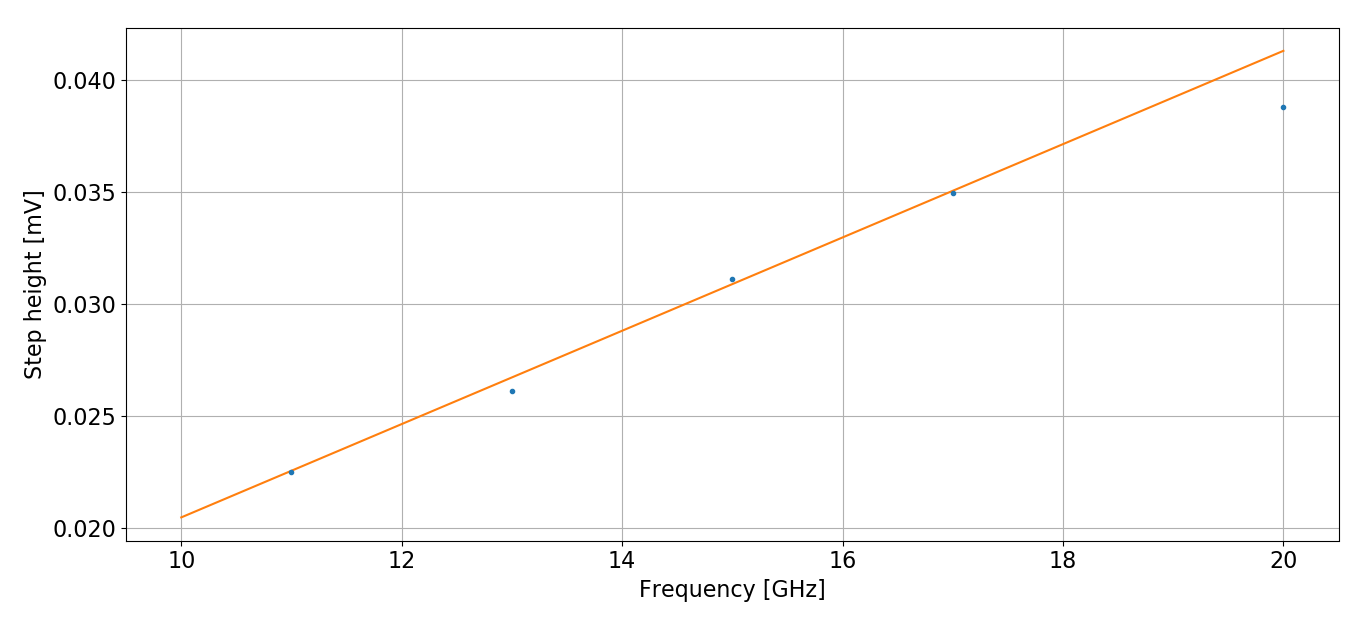
\includegraphics[width = \textwidth]{eh}
\caption{Step height as a function of frequency, orange line is the linear regression. Errors on the point are too small to be seen}\label{eh}
\end{figure}
\subsection{Critical temperature measurement}

\begin{thebibliography}{99}
\bibitem{firstsuperconductor} \textsc{H. K. Onnes} \textit{The resistance of pure mercury at helium temperatures}, Commun. Phys. Lab. Univ. Leiden, Vol. 12 (1911), 120 

\bibitem{skriptum}
STAR Cryoelectronics, \textit{Mr. SQUID User's  Guide}. \textsc{Randy W. Simon, Michael J. Burns, Mark S. Colclough, Greg Zaharchuk, Robin Cantor}. 

\bibitem{grossmarx}
De Gruyter Studium, \textit{Festkörperphysik}. \textsc{Rudolf Gross, Achim Marx}. 3. Edition.

\bibitem{squid_circuit}
Wikimedia, \textsc{Jan Olaf}. \url{https://upload.wikimedia.org/wikipedia/commons/7/71/SQUID_IV.jpg}.

\bibitem{datasheet}
STAR Cryoelectronics, \textit{Mr. SQUID Datasheet}. \textsc{R. Cantor}. 

\end{thebibliography}
\end{document}
